%Version 3.1 December 2024
% See section 11 of the User Manual for version history
%
%%%%%%%%%%%%%%%%%%%%%%%%%%%%%%%%%%%%%%%%%%%%%%%%%%%%%%%%%%%%%%%%%%%%%%
%%                                                                 %%
%% Please do not use \input{...} to include other tex files.       %%
%% Submit your LaTeX manuscript as one .tex document.              %%
%%                                                                 %%
%% All additional figures and files should be attached             %%
%% separately and not embedded in the \TeX\ document itself.       %%
%%                                                                 %%
%%%%%%%%%%%%%%%%%%%%%%%%%%%%%%%%%%%%%%%%%%%%%%%%%%%%%%%%%%%%%%%%%%%%%

%%\documentclass[referee,sn-basic]{sn-jnl}% referee option is meant for double line spacing

%%=======================================================%%
%% to print line numbers in the margin use lineno option %%
%%=======================================================%%

\documentclass[lineno,pdflatex,sn-nature]{sn-jnl}% Basic Springer Nature Reference Style/Chemistry Reference Style

%%=========================================================================================%%
%% the documentclass is set to pdflatex as default. You can delete it if not appropriate.  %%
%%=========================================================================================%%

%%\documentclass[sn-basic]{sn-jnl}% Basic Springer Nature Reference Style/Chemistry Reference Style

%%Note: the following reference styles support Namedate and Numbered referencing. By default the style follows the most common style. To switch between the options you can add or remove “Numbered” in the optional parenthesis. 
%%The option is available for: sn-basic.bst, sn-chicago.bst%  
 
%%\documentclass[pdflatex,sn-nature]{sn-jnl}% Style for submissions to Nature Portfolio journals
%%\documentclass[pdflatex,sn-basic]{sn-jnl}% Basic Springer Nature Reference Style/Chemistry Reference Style
%%\documentclass[pdflatex,sn-mathphys-num]{sn-jnl}% Math and Physical Sciences Numbered Reference Style
%%\documentclass[pdflatex,sn-mathphys-ay]{sn-jnl}% Math and Physical Sciences Author Year Reference Style
%%\documentclass[pdflatex,sn-aps]{sn-jnl}% American Physical Society (APS) Reference Style
%%\documentclass[pdflatex,sn-vancouver-num]{sn-jnl}% Vancouver Numbered Reference Style
%%\documentclass[pdflatex,sn-vancouver-ay]{sn-jnl}% Vancouver Author Year Reference Style
%%\documentclass[pdflatex,sn-apa]{sn-jnl}% APA Reference Style
%%\documentclass[pdflatex,sn-chicago]{sn-jnl}% Chicago-based Humanities Reference Style

%%%% Standard Packages
%%<additional latex packages if required can be included here>

\usepackage{graphicx}%
\usepackage{multirow}%
\usepackage{amsmath,amssymb,amsfonts}%
\usepackage{amsthm}%
\usepackage{mathrsfs}%
\usepackage[title]{appendix}%
\usepackage{xcolor}%
\usepackage{textcomp}%
\usepackage{manyfoot}%
\usepackage{booktabs}%
\usepackage{algorithm}%
\usepackage{algorithmicx}%
\usepackage{algpseudocode}%
\usepackage{listings}%

%%%%

%%%%%=============================================================================%%%%
%%%%  Remarks: This template is provided to aid authors with the preparation
%%%%  of original research articles intended for submission to journals published 
%%%%  by Springer Nature. The guidance has been prepared in partnership with 
%%%%  production teams to conform to Springer Nature technical requirements. 
%%%%  Editorial and presentation requirements differ among journal portfolios and 
%%%%  research disciplines. You may find sections in this template are irrelevant 
%%%%  to your work and are empowered to omit any such section if allowed by the 
%%%%  journal you intend to submit to. The submission guidelines and policies 
%%%%  of the journal take precedence. A detailed User Manual is available in the 
%%%%  template package for technical guidance.
%%%%%=============================================================================%%%%

%% as per the requirement new theorem styles can be included as shown below
\theoremstyle{thmstyleone}%
\newtheorem{theorem}{Theorem}%  meant for continuous numbers
%%\newtheorem{theorem}{Theorem}[section]% meant for sectionwise numbers
%% optional argument [theorem] produces theorem numbering sequence instead of independent numbers for Proposition
\newtheorem{proposition}[theorem]{Proposition}% 
%%\newtheorem{proposition}{Proposition}% to get separate numbers for theorem and proposition etc.

\theoremstyle{thmstyletwo}%
\newtheorem{example}{Example}%
\newtheorem{remark}{Remark}%

\theoremstyle{thmstylethree}%
\newtheorem{definition}{Definition}%

\raggedbottom
%%\unnumbered% uncomment this for unnumbered level heads

\begin{document}

\title[Article Title]{Quantifying superspreading in bacterial STI outbreaks using phylodynamics}



%%=============================================================%%
%% GivenName	-> \fnm{Joergen W.}
%% Particle	-> \spfx{van der} -> surname prefix
%% FamilyName	-> \sur{Ploeg}
%% Suffix	-> \sfx{IV}
%% \author*[1,2]{\fnm{Joergen W.} \spfx{van der} \sur{Ploeg} 
%%  \sfx{IV}}\email{iauthor@gmail.com}
%%=============================================================%%

\author[1]{\fnm{Jordi}\sur{Sevilla-Fortuny}}\email{jordi.sevilla-fortuny@pasteur.fr}

\author[1]{\fnm{Julia}\sur{Kende}}\email{}

\author[]{\fnm{Michael}\sur{Meehan}}\email{}

\author[]{\fnm{Timothy}\sur{Vaughan}}\email{}

\author*[1]{\fnm{Sebastian}\sur{Duchêne}}\email{}


\affil[1]{\orgdiv{Computational Biology}, \orgname{Institut Pasteur}, \orgaddress{\street{Rue Du Dr Roux}, \postcode{75015}, \state{Paris}, \country{France}}}


\maketitle

\section*{Supplementary File}\label{sec1}


\begin{figure}[H]
    \centering
    \title{Suplementary figure 1}
    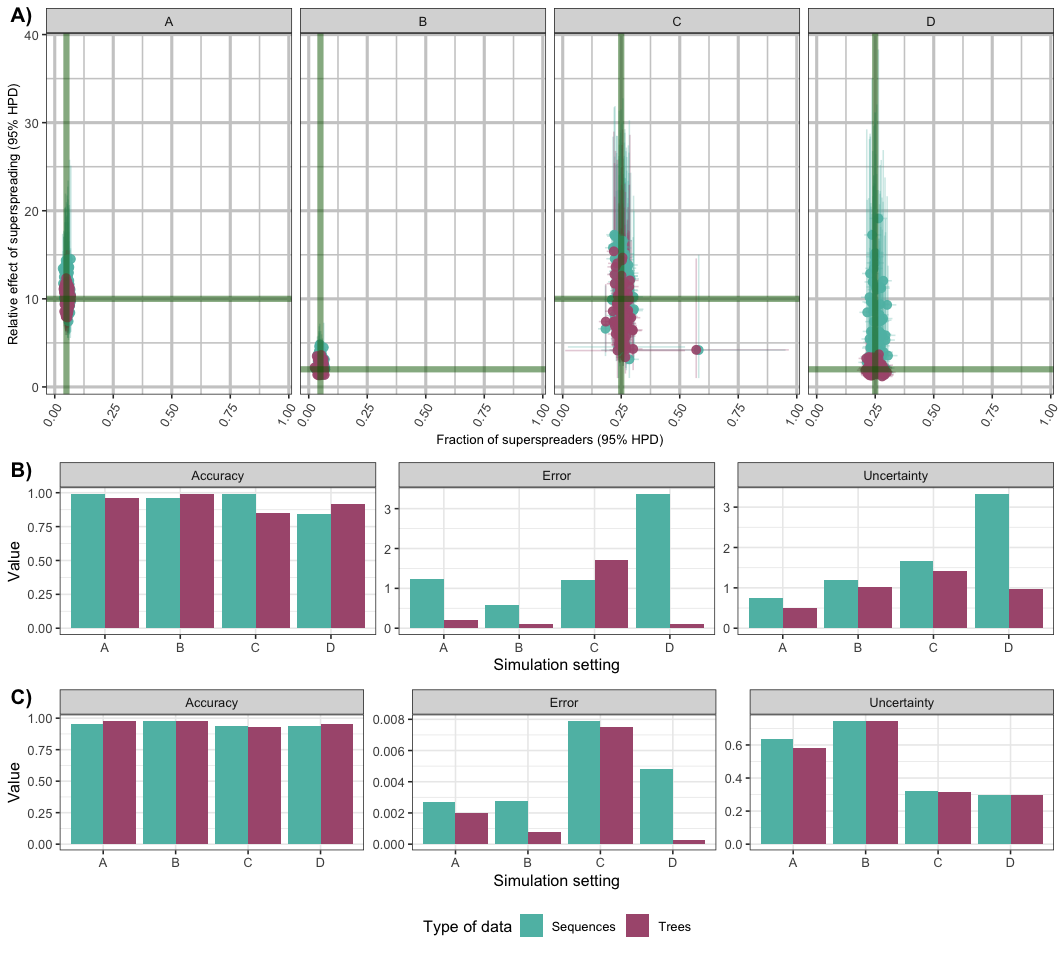
\includegraphics[width=1\linewidth]{figures/sup_figures/Simulations_tiptypes.png}
    \caption{Performance of superspreading inference under varying simulation conditions with known tip-types. A) Posterior means and 95\% highest posterior density (HPD) intervals for the fraction of superspreaders ($f_{ss}$, x-axis) and their transmission advantage ($\mathcal{T}_a$,y-axis). Panels correspond to different simulation settings (A–D). Points represent posterior summaries, and colours indicate the data type used for inference (trees vs. sequences). Green lines denote the true simulated values. B–C) Accuracy, error, and uncertainty of parameter estimates across simulation settings. B) Transmission advantage. C) Fraction of superspreaders. Colours indicate the data type used (trees vs. sequences).}
    \label{fig-simulations}
\end{figure}

\begin{figure}[H]
    \centering
    \title{Suplementary figure 2}
    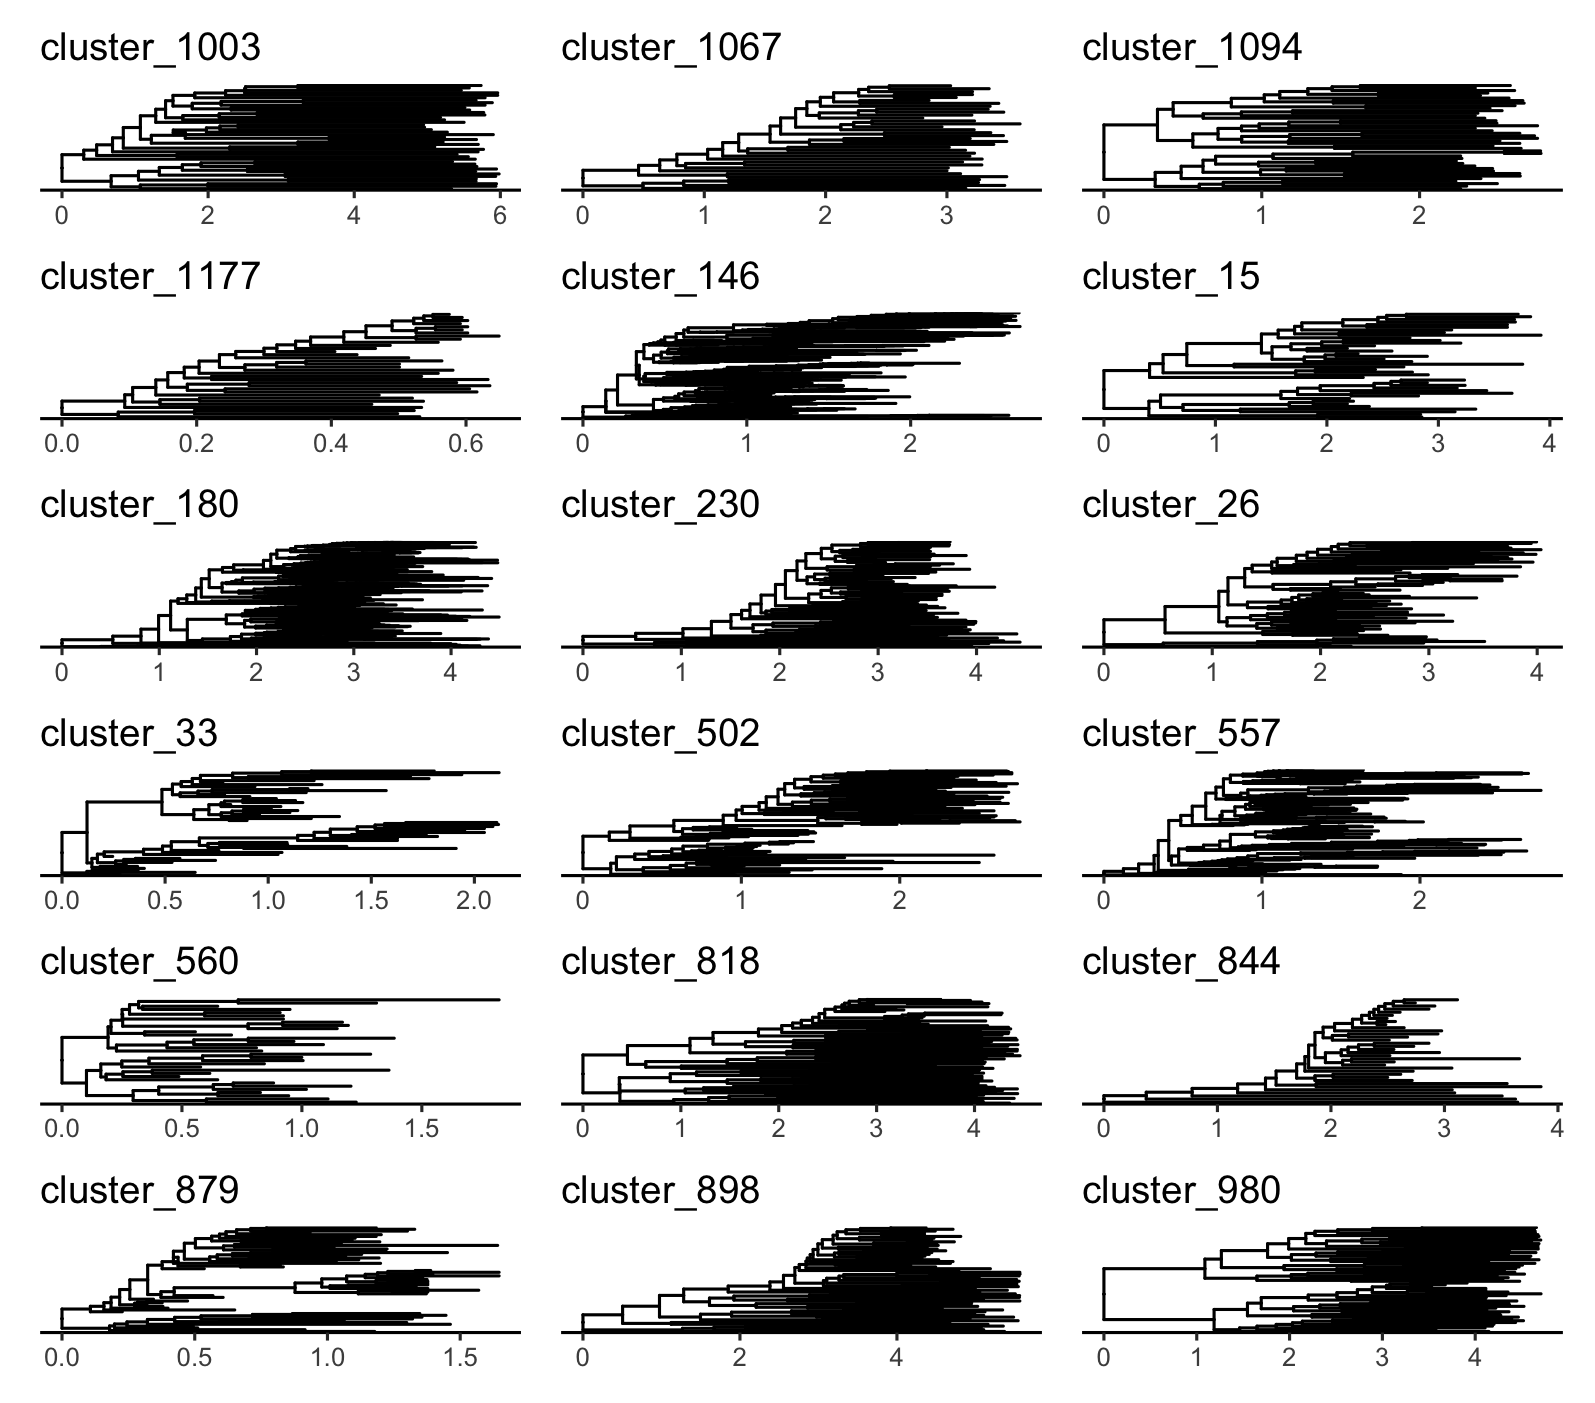
\includegraphics[width=1\linewidth]{figures/sup_figures/Tree_figure.png}
    \caption{Maximum clade credibility trees for the clusters analysed}
    \label{fig-simulations}
\end{figure}

\begin{figure}[H]
    \centering
    \title{Suplementary figure 3}
    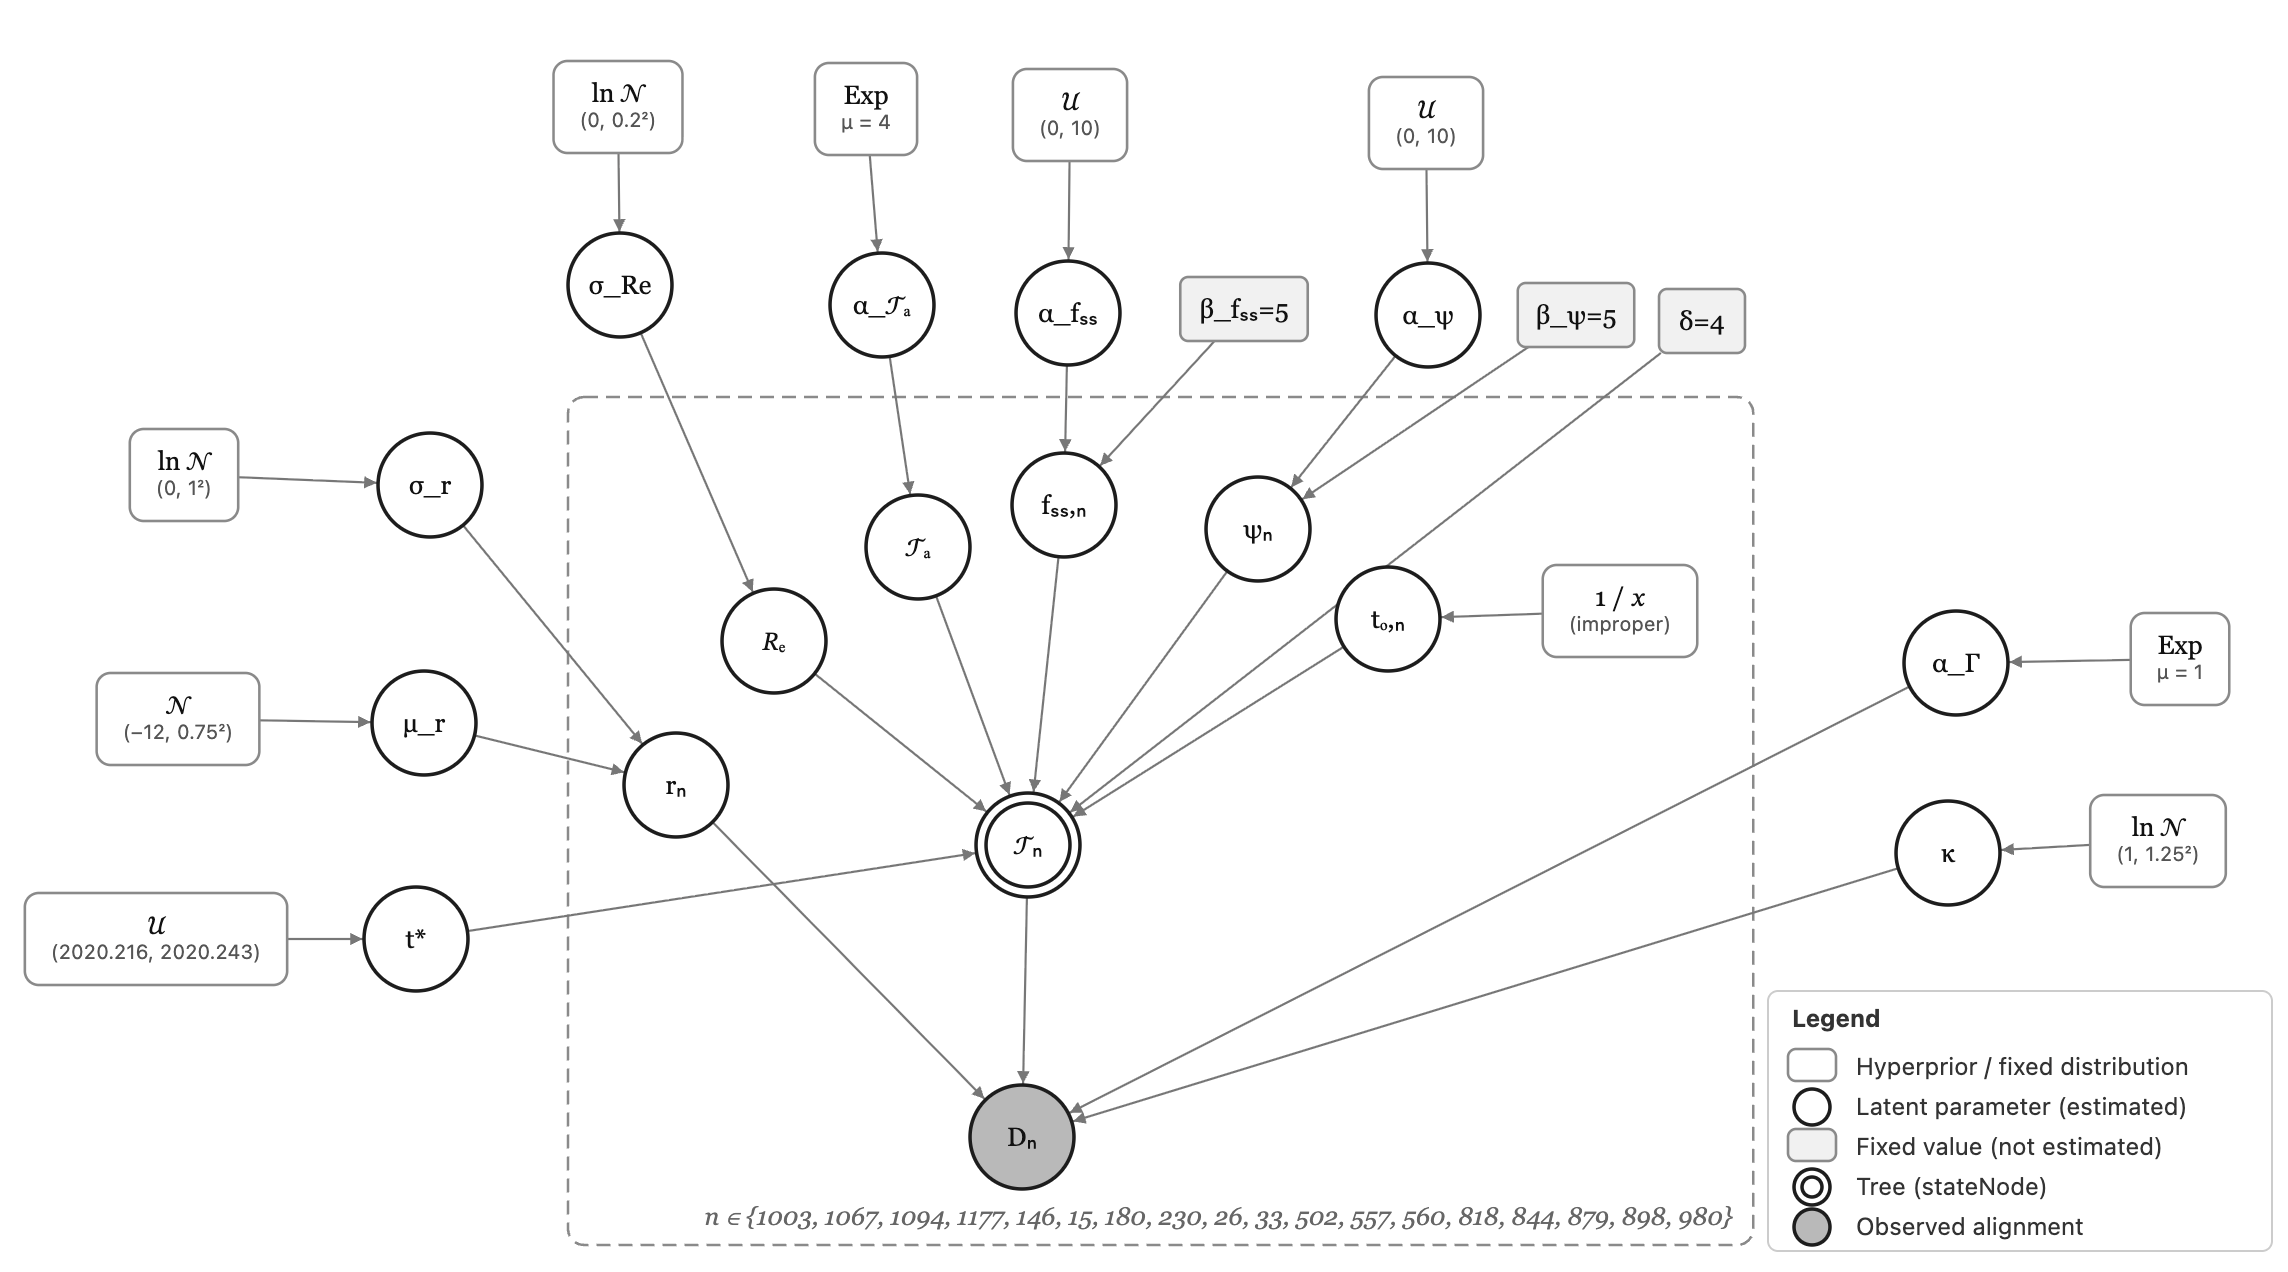
\includegraphics[width=1\linewidth]{figures/sup_figures/plate.png}
    \caption{Plate diagram of the hierarchical model used to analyze the real \textit{N. gonorrhoeae} data}
    \label{fig-diagram}
\end{figure}

\begin{figure}[H]
    \centering
    \title{Suplementary figure 4}
    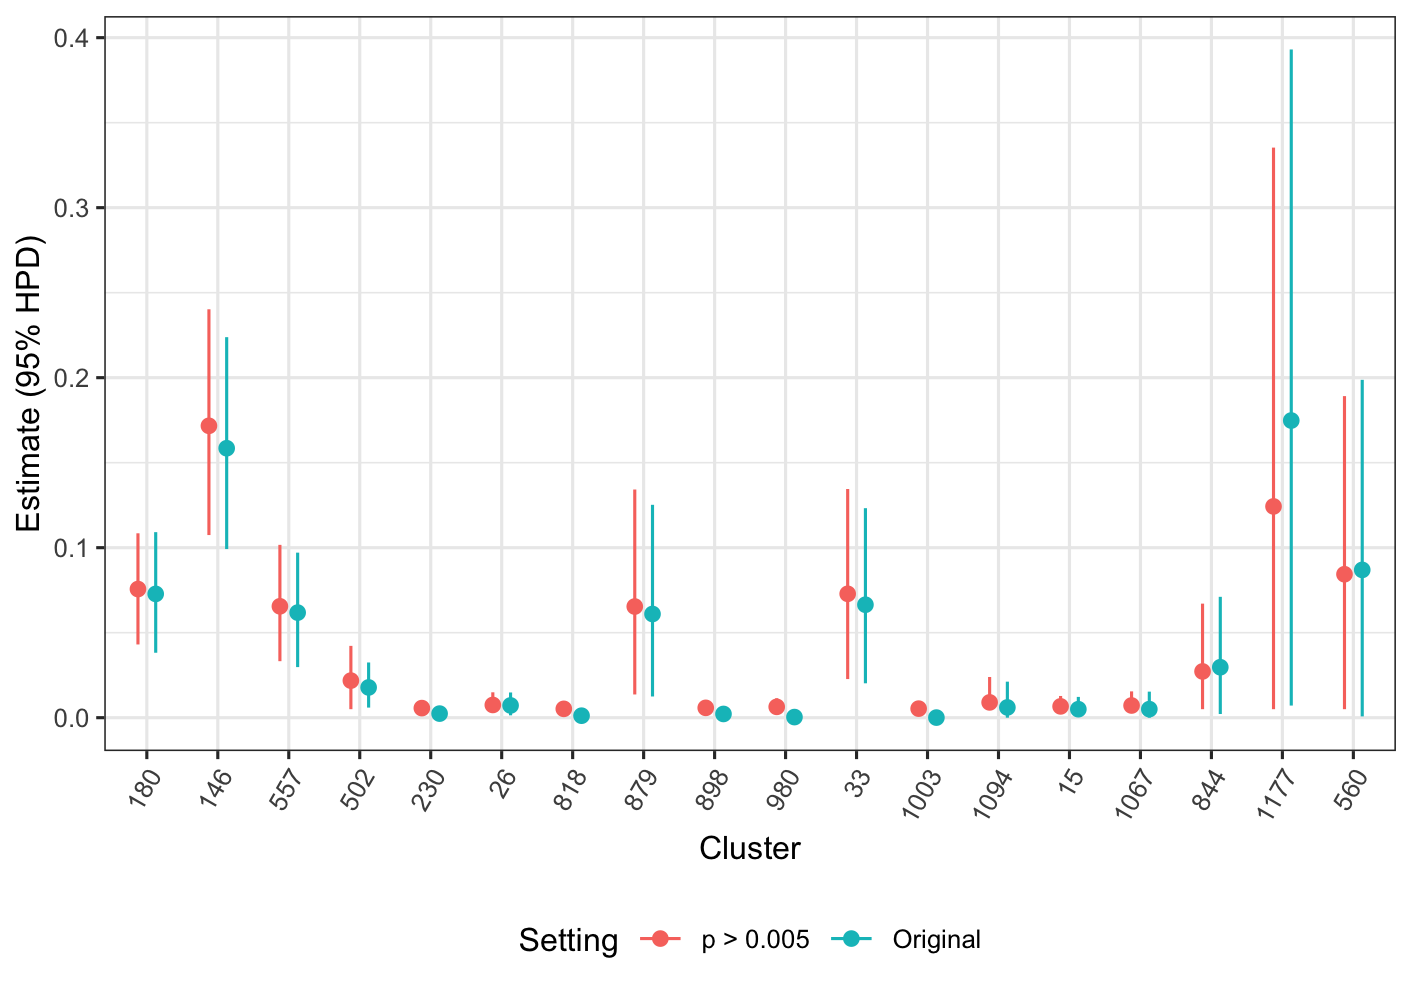
\includegraphics[width=1\linewidth]{figures/sup_figures/comparision_sampling_proportion.png}
    \caption{Estimates and 95\% HPD intervals of the sampling proportion for each analyzed cluster. Blue points correspond to the original inference described in the manuscript, whereas red points correspond to the inference obtained when the sampling proportion was constrained to be greater than 0.005.}
    \label{fig-second-run}
\end{figure}

\end{document}


